\chapter{Software Umsetzung}

Das Projekt stellte für uns nicht nur in Bezug auf die Hardware hohe Anforderungen, sondern erforderte auch für ein Mikrocontroller-Projekt eine ungewöhnlich komplexe Softwarelösung. Von Beginn an war es daher essenziell, eine klare und gut organisierte Struktur zu etablieren. Diese Vorgehensweise gewährleistet, dass der Code sowohl wartbar als auch übersichtlich bleibt, was für die effiziente Entwicklung des Projekts von großer Bedeutung ist.

Des Weiteren wurde von Beginn an besonderer Wert darauf gelegt, den Code unter Versionskontrolle zu stellen, wofür Git gewählt wurde. Dieser Schritt gewährleistete eine effiziente Verwaltung der Code-Änderungen und bot eine robuste Plattform für die Zusammenarbeit im Team an.

\section{Entwicklungsumgebung}

Für die Entwicklung der Software wurde Visual Studio Code (VSCode) als integrierte Entwicklungsumgebung (IDE) ausgewählt. VSCode ist aufgrund seiner vielseitigen Fähigkeiten hervorragend für die Programmierung von Mikrocontrollern geeignet. Diese Plattform zeichnet sich durch eine Vielzahl an Erweiterungen (Plugins) aus, die speziell für verschiedene Programmiersprachen und Projektspezifikationen konzipiert sind. Diese Flexibilität und Anpassungsfähigkeit von VSCode macht es zu einem idealen Werkzeug auch für dieses Entwicklungsprojekt.

\section{Programmiersprache}

Aufgrund der Nutzung des Arduino Uno als Mikrocontroller fiel die Wahl für die Entwicklungssprache auf C++. Arduino zeichnet sich durch seine umfangreichen Bibliotheken aus, die die Integration von Funktionen und Komponenten erheblich erleichtern. Diese Bibliotheken bieten eine reiche Auswahl an vorgefertigten Codes und Modulen, die es ermöglichen, komplexe Funktionen mit geringerem Aufwand zu implementieren und somit die Entwicklungszeit zu verkürzen. 

\section{PlatformIO}

Wie bereits erwähnt, zeichnet sich Visual Studio Code durch seine umfangreiche Plugin-Unterstützung aus. Für dieses Projekt wurde speziell das Plugin PlatformIO verwendet, das sich als äußerst nützlich für die Arbeit mit Mikrocontrollern erwiesen hat. PlatformIO bietet umfassende Unterstützung bei der Handhabung des Arduino Uno. Es ermöglicht nicht nur das Kompilieren des Codes, sondern auch das bequeme Übertragen auf den Mikrocontroller. Zudem bietet es die Möglichkeit, verschiedene Ausgaben über den Serial Monitor zu überwachen.

Ein zentrales Element von PlatformIO ist die 'platformio.ini'-Datei. In dieser Konfigurationsdatei werden wichtige Projektinformationen festgelegt, wie zum Beispiel der verwendete Mikrocontroller-Typ (Arduino Uno), das Framework (Arduino) und die eingebundenen Bibliotheken.

\begin{figure}[H]
    \centerline{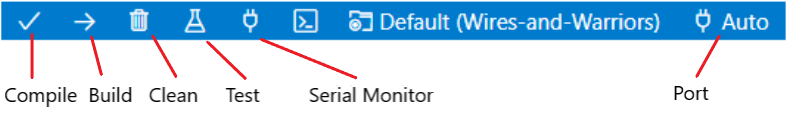
\includegraphics[width=.85\textwidth,scale=1]{./images/platformio.png}}
    \caption{PlatformIO Unterstützung in VSCode}\label{herzen}
\end{figure}

\section{Komponenten}

Bei der Entwicklung wurde ein besonderes Augenmerk einen fein gegliederten und modularen Codeaufbau gelegt. Um diesen modularen Ansatz zu unterstützen, wurde für jede Komponente (repräsentiert durch eine .cpp-Datei) eine zugehörige Header-Datei (.h) erstellt. In diesen Header-Dateien sind alle nach außen sichtbaren Methoden und Variablen der jeweiligen Komponente definiert. Dies fördert eine klare Trennung zwischen der Implementierung und der Schnittstellendefinition, was die Lesbarkeit und Wartbarkeit des Codes wesentlich verbessert.

Die Applikation wurde in folgende Hauptkomponenten unterteilt: 

\subsection{main}

Die main.cpp dient als zentrale Datei der Applikation. Ihre Hauptfunktion besteht darin, verschiedene Services und Module zu initialisieren. Zusätzlich beinhaltet die main.cpp spezifische Funktionen für Arduino, wie:

\begin{minipage}{\linewidth}
\begin{lstlisting}
void setup() { ... }
void loop() { ... }
\end{lstlisting}
\end{minipage}

\subsection{Game}

Die Game-Komponente stellt den umfassendsten Teil der gesamten Applikation dar. Sie beinhaltet die vollständige Logik, die den Zustand (State) und den Ablauf des Spiels bestimmt.

In jedem Zyklus (Tick) des Spiels wird die dazugehörige Funktion der Komponente aufgerufen. Diese Funktion übernimmt essentielle Aufgaben wie die korrekte Steuerung der LED-Anzeigen oder das Auslösen von Bewegungen der Motoren. Zusätzlich dazu beinhaltet die Game-Komponente wichtige Funktionen, die das Level-System des Spiels betreffen, wie beispielsweise die Fortschrittsverwaltung oder die Schwierigkeitssteigerung.

Hier ein vereinfachter Überblick über die Hauptfunktion dieser Komponente:

\begin{minipage}{\linewidth}
\begin{lstlisting}
// simplified version
void tick() {
    showHeartLights();

    if (checkWireTouch()) { ... }
    
    if (gameStarted) {
        turnBridge();
    }
}
\end{lstlisting}
\end{minipage}

\subsection{gameConstants}

Diese Komponente beinhaltet eine Sammlung von Konstanten, die sowohl für das Design des Spiels als auch für dessen Dynamik von entscheidender Bedeutung sind. Diese Konstanten umfassen sowohl feste Parameter, die das grundlegende Erscheinungsbild und Verhalten des Spiels definieren, als auch variierbare Elemente, die es ermöglichen, den Spielfluss sowie visuelle und auditive Effekte anzupassen. Die Flexibilität dieser Konstanten ermöglicht es den Entwicklern, mit verschiedenen Spielaspekten zu experimentieren und das Spielerlebnis zu optimieren.

Nachfolgend finden Sie einen nicht vollständigen Auszug aus dieser Sektion:

\begin{minipage}{\linewidth}
\begin{lstlisting}
// fixed values
const int lifeLEDsCount = 6;
const int pulsesForFullRotation = 6400; // motor specific

// variable values
const int errorCooldown = 1000; // milliseconds
const int volume = 25; // 0-30
\end{lstlisting}
\end{minipage}

\subsection{lights}

Die lights-Komponente ist für die Kontrolle sämtlicher Beleuchtungselemente im Spiel zuständig. Ein wesentlicher Bestandteil dieser Komponente sind die Start- und End-LEDs, welche als feste grüne LEDs an den Türmen integriert sind.

Das zweite zentrale Element der lights-Komponente sind die LEDs für die Darstellung der Herzen. Diese sind als smarte LEDs konzipiert, was bedeutet, dass sie in der Lage sind, verschiedene Farben anzunehmen. Die Farbänderungen erfolgen entsprechend dem aktuellen Zustand (State) im Spielverlauf. 

Für die Ansteuerung der Herzen-LEDs wird die Adafruit\_NeoPixel-Bibliothek verwendet. Diese Bibliothek bietet eine umfangreiche Palette an Funktionen für die Kontrolle von RGB-LEDs.

Einige der Funktionen der lights-Komponente umfassen:

\begin{minipage}{\linewidth}
\begin{lstlisting}
void showGameNotStarted() { ... }
void showHearts(int playerHeartCount) { ... }
void showError(int lastError) { ... }
void showRingLights() { ... }
\end{lstlisting}
\end{minipage}    

\subsection{logging}

Die Logging-Komponente ist ausschließlich für Debugging-Zwecke konzipiert. Ihr Hauptmerkmal ist eine globale Log-Funktion, die für die Protokollierung von Informationen während der Entwicklungs- und Testphasen des Spiels verwendet wird. Diese Funktion nutzt den Standardmechanismus des Serial Monitors, um Log-Nachrichten auszugeben, mit dem einzigen Unterschied, dass eine Überprüfung stattfindet, ob die Logging-Funktion aktiviert ist, bevor irgendwelche Nachrichten protokolliert werden.

\subsection{motor}

Die motor-Komponente ist zuständig für die Steuerung aller Motoren im Spiel. Sie umfasst sowohl die Kontrolle des Motors für das Brückenelement als auch die Ansteuerung der Motoren, welche die Drähte an den Türmen bewegen.

Außerdem ein wichtiger Bestandteil dieser Komponente sind die Überprüfungsfunktionen, die kontrollieren, ob und wann eine Drehung der Motoren durchgeführt werden soll. Details dazu werden später genauer erläutert.

Als Beispiel für die Funktionalität dieser Komponente dient die Funktion zum Drehen der Turmdrähte:

\begin{minipage}{\linewidth}
\begin{lstlisting}
void turnSides(int level) {
    if (!timeToTurnSides()) {
        return;
    }

    for (int i = 0; i < getMotorRotations(level); i++) {
        // turn side motors one step
        digitalWrite(stepPinWire, HIGH);
        delayMicroseconds(1); // we need the delay
        digitalWrite(stepPinWire, LOW);
    }
}
\end{lstlisting}
\end{minipage}  


\subsection{pins}
Die pins-Datei spielt eine wesentliche Rolle in der Organisation und Konfiguration des Projekts, indem sie eine klare und strukturierte Übersicht über die Belegung aller Pins bietet. In dieser Datei werden alle Pins, die für die Verbindung des Arduino-Boards mit den verschiedenen Komponenten des Systems verwendet werden, über Konstanten definiert.

Diese systematische Zuordnung ist besonders hilfreich während der Verkabelungsphase, da sie eine genaue und fehlerfreie Verbindung der Hardware-Komponenten mit den entsprechenden Pins des Arduino-Boards gewährleistet. Änderungen in der Hardware-Konfiguration können somit leichter umgesetzt werden, indem die entsprechenden Werte in der pins-Datei angepasst werden, ohne den Hauptcode des Projekts zu beeinflussen.

\subsection{touch}
Diese Komponente ist eine unterstützende Funktionseinheit, die speziell für die Erkennung von Berührungen an bestimmten Pins konzipiert wurde. Diese Funktion ist ein kritischer Bestandteil des Spiels und wird in verschiedenen Szenarien eingesetzt, wie beispielsweise beim Start des Spiels, beim Erreichen des Ziels oder bei der Erkennung eines Fehlers, also einer Berührung des Drahtes.

Die Kernfunktion der touch-Komponente nutzt die digitalRead()-Funktion, die von der Arduino-Bibliothek bereitgestellt wird.

\begin{minipage}{\linewidth}
\begin{lstlisting}
bool playerTouchesPin(int pin) {
    return !digitalRead(pin);
}
\end{lstlisting}
\end{minipage}

\section{Asynchronität der Software}

Die Herausforderung, mehrere Funktionen gleichzeitig auszuführen, war ein komplexes Problem im Rahmen dieses Projekts. Insbesondere mussten die Motoren kontinuierlich laufen, während das Spiel fortschritt, Berechnungen durchgeführt und ständig auf Berührungen geprüft wurden.
Dies stellte sich als besonders schwierig heraus, da außerdem im Spiel zahlreiche zeitbasierte Funktionen existieren, wie etwa Fehler-Cooldowns mit Animationen sowie Start- und Endanimationen für jedes Level.

Anfangs wurde versucht, das Problem mit Verzögerungen (Delays) im Code zu lösen. Diese Methode führte jedoch zu nicht nachhaltigen Lösungen und verursachte während der Entwicklung immer wieder Bugs.
Die endgültige Lösung des Problems fand sich in der Verwendung von Zeitstempeln. An verschiedenen Stellen in der Anwendung wird ein Zeitstempel gesetzt und anschließend überprüft, ob eine bestimmte Zeitspanne verstrichen ist.

Diese Methode ermöglicht es, eine Art von Asynchronität zu simulieren. Durch das Arbeiten mit Zeitstempeln statt festen Verzögerungen kann das Programm fortlaufend andere wichtige Aufgaben ausführen, während es gleichzeitig auf das Erreichen bestimmter Zeitpunkte wartet. Dieser Ansatz verbessert nicht nur die Ansprechbarkeit (Reaktion) des Programms, sondern erhöht auch die Stabilität und Zuverlässigkeit des Codes, indem er die typischen Probleme vermeidet, die mit der Verwendung von Delays einhergehen.

\subsection{Beispiel}

Dieses Vorgehen lässt sich gut am Beispiel der Funktionalität zum Drehen des Brückenmotors illustrieren. Die turnBridge()-Funktion beginnt mit einer Überprüfung, ob eine Drehung der Brücke überhaupt möglich ist. Diese Überprüfung wird durch die Funktion timeToTurnBridge() realisiert, die auf Zeitsteuerung basiert. Es wird kontrolliert, ob die festgelegte Zeitspanne seit dem letzten Aktivieren der Brückendrehung verstrichen ist. Sobald festgestellt wird, dass die definierte Zeitspanne abgelaufen ist, wird der Brückenmotor aktiviert und der Zeitstempel aktualisiert, um den nächsten Zeitpunkt für eine mögliche Aktivierung zu markieren.

\begin{minipage}{\linewidth}
\begin{lstlisting}
// vereinfachte version
void turnBridge() {
    if (!timeToTurnBridge()) {
        return;
    }
    
    ...
}

bool timeToTurnBridge() {
    bool timeToTurn = elapsedTime >= motorDelay;

    if (timeToTurn) {
        lastBridgeTurnTime = currentTime;
    }

    return timeToTurn;
}
\end{lstlisting}
\end{minipage}